\documentclass[tikz,border=8pt]{standalone}
\usepackage{fontspec}
\usepackage{graphicx}
\usepackage{amssymb}
\setmainfont{Latin Modern Roman}
\usetikzlibrary{arrows.meta,positioning,calc,fit,backgrounds}

\definecolor{waveblue}{RGB}{219,237,252}
\definecolor{freqorange}{RGB}{255,231,199}
\definecolor{embedgreen}{RGB}{220,243,224}
\definecolor{modelpurple}{RGB}{235,224,249}
\definecolor{headgray}{RGB}{233,236,240}
\definecolor{preyellow}{RGB}{250,244,204}

\tikzset{
  box/.style={
    draw,
    rounded corners=2pt,
    minimum height=11mm,
    minimum width=29mm,
    text width=31mm,
    inner sep=3.2pt,
    align=center,
    font=\sffamily\small,
    line width=0.55pt
  },
  input/.style={box,fill=preyellow},
  wave/.style={box,fill=waveblue},
  freq/.style={box,fill=freqorange},
  embed/.style={box,fill=embedgreen},
  model/.style={box,fill=modelpurple,minimum height=23mm,text width=35mm},
  head/.style={box,fill=headgray},
  sum/.style={circle,draw,line width=0.65pt,minimum size=9mm,
              inner sep=0pt,font=\sffamily\bfseries\large,fill=white},
  flow/.style={-{Latex[length=2.2mm]},line width=0.7pt},
  guide/.style={-{Latex[length=2mm]},line width=0.55pt},
  optional/.style={-{Latex[length=2mm]},line width=0.55pt,dashed},
  note/.style={font=\sffamily\scriptsize,align=center,text=black!68},
  group/.style={draw=black!30,rounded corners=4pt,dashed,inner sep=5pt}
}

\begin{document}

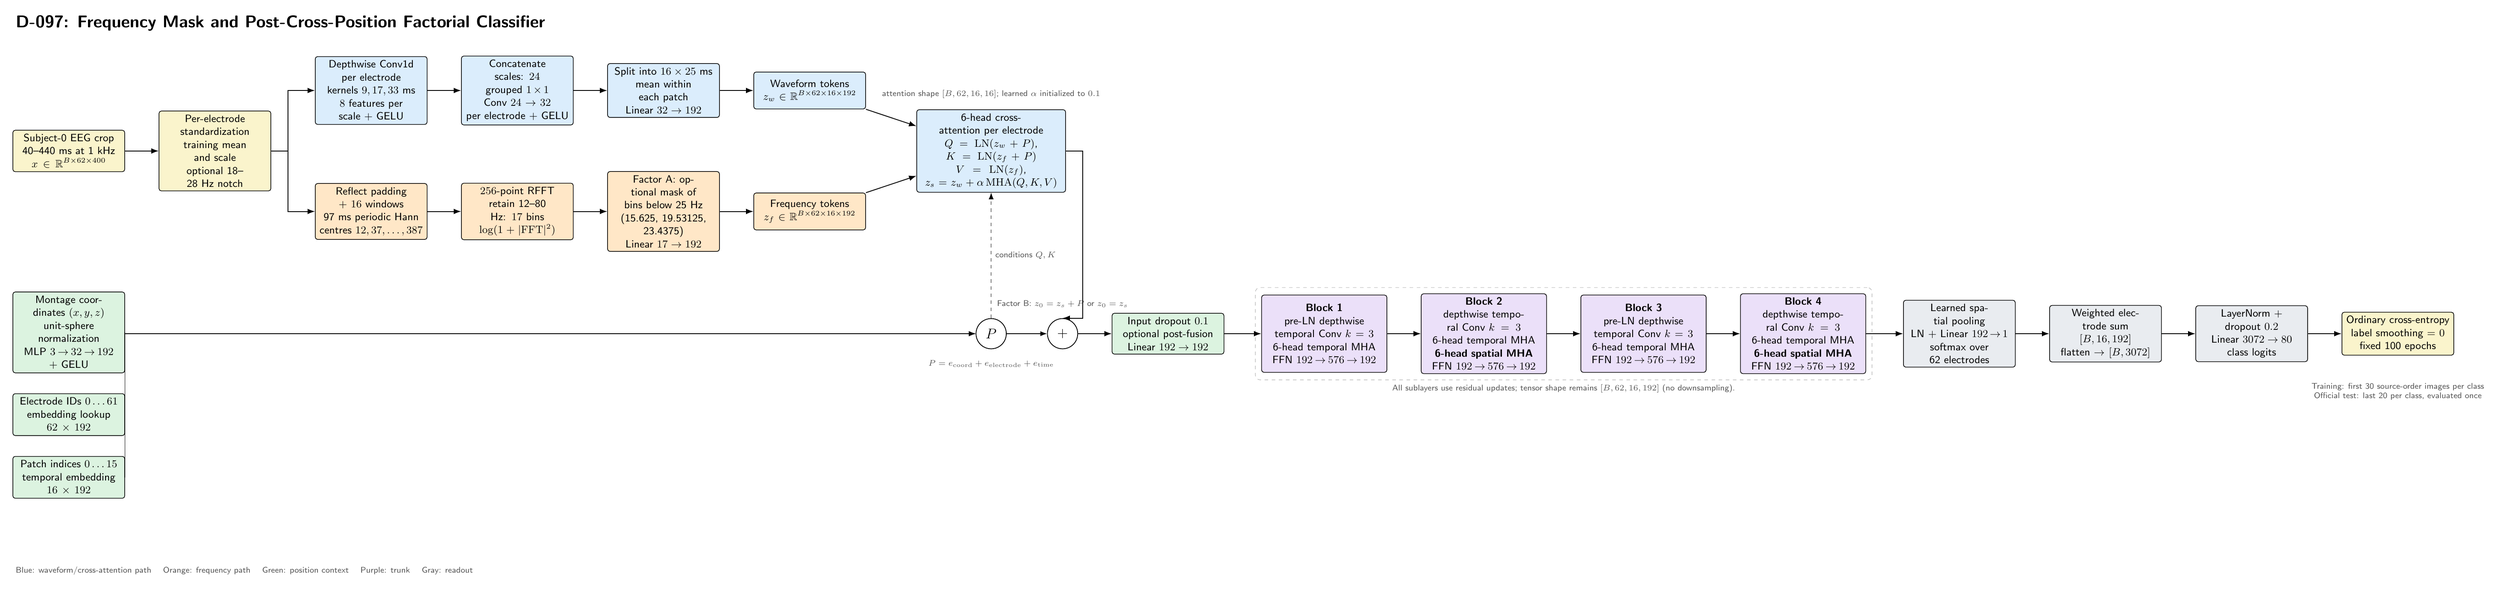
\begin{tikzpicture}[node distance=9mm and 10mm]
  \node[font=\sffamily\bfseries\Large,anchor=west] at (-1.7,6.2)
    {D-097: Frequency Mask and Post-Cross-Position Factorial Classifier};

  % Shared input and preprocessing.
  \node[input] (raw) at (0,2.4)
    {Subject-0 EEG crop\\40--440 ms at 1 kHz\\$x\in\mathbb{R}^{B\times62\times400}$};
  \node[input,right=of raw] (prep)
    {Per-electrode standardization\\training mean and scale\\optional 18--28 Hz notch};
  \draw[flow] (raw) -- (prep);

  % Waveform branch.
  \node[wave,right=13mm of prep,yshift=18mm] (wconv)
    {Depthwise Conv1d per electrode\\kernels $9,17,33$ ms\\$8$ features per scale + GELU};
  \node[wave,right=of wconv] (wcat)
    {Concatenate scales: $24$\\grouped $1\!\times\!1$ Conv $24\!\to\!32$\\per electrode + GELU};
  \node[wave,right=of wcat] (wpatch)
    {Split into $16\times25$ ms\\mean within each patch\\Linear $32\!\to\!192$};
  \node[wave,right=of wpatch] (zw)
    {Waveform tokens\\$z_w\in\mathbb{R}^{B\times62\times16\times192}$};
  \draw[flow] (prep.east) -- ++(5mm,0) |- (wconv.west);
  \draw[flow] (wconv) -- (wcat);
  \draw[flow] (wcat) -- (wpatch);
  \draw[flow] (wpatch) -- (zw);

  % Frequency branch.
  \node[freq,right=13mm of prep,yshift=-18mm] (fwin)
    {Reflect padding + $16$ windows\\97 ms periodic Hann\\centres $12,37,\ldots,387$};
  \node[freq,right=of fwin] (fft)
    {$256$-point RFFT\\retain 12--80 Hz: $17$ bins\\$\log(1+|\mathrm{FFT}|^2)$};
  \node[freq,right=of fft] (fproj)
    {Factor A: optional mask of bins below 25 Hz\\(15.625, 19.53125, 23.4375)\\Linear $17\!\to\!192$};
  \node[freq,right=of fproj] (zf)
    {Frequency tokens\\$z_f\in\mathbb{R}^{B\times62\times16\times192}$};
  \draw[flow] (prep.east) -- ++(5mm,0) |- (fwin.west);
  \draw[flow] (fwin) -- (fft);
  \draw[flow] (fft) -- (fproj);
  \draw[flow] (fproj) -- (zf);

  % Directional cross-attention fusion.
  \node[wave,text width=42mm,right=15mm of zw,yshift=-18mm] (gate)
    {6-head cross-attention per electrode\\$Q=\mathrm{LN}(z_w+P)$, $K=\mathrm{LN}(z_f+P)$\\$V=\mathrm{LN}(z_f)$, $z_s=z_w+\alpha\,\mathrm{MHA}(Q,K,V)$};
  \node[note,above=2mm of gate] {attention shape $[B,62,16,16]$; learned $\alpha$ initialized to $0.1$};
  \draw[flow] (zw) -- (gate);
  \draw[flow] (zf) -- (gate);

  % Embedding construction.
  \node[embed] (coord) at (0,-3.0)
    {Montage coordinates $(x,y,z)$\\unit-sphere normalization\\MLP $3\!\to\!32\!\to\!192$ + GELU};
  \node[embed,below=6mm of coord] (eid)
    {Electrode IDs $0\ldots61$\\embedding lookup\\$62\times192$};
  \node[embed,below=6mm of eid] (tid)
    {Patch indices $0\ldots15$\\temporal embedding\\$16\times192$};

  \node[sum] (pos) at ($(gate.south)+(0,-42mm)$) {$P$};
  \node[note,below=2mm of pos]
    {$P=e_{\mathrm{coord}}+e_{\mathrm{electrode}}+e_{\mathrm{time}}$};
  \draw[guide] (coord.east) |- (pos.west);
  \draw[guide] (eid.east) |- (pos.west);
  \draw[guide] (tid.east) |- (pos.west);
  \draw[optional] (pos.north) -- node[note,right]{conditions $Q,K$} (gate.south);

  \node[sum,right=12mm of pos] (add) {$+$};
  \node[note,above=2mm of add] {Factor B: $z_0=z_s+P$ or $z_0=z_s$};
  \draw[flow] (gate.east) -- ++(5mm,0) |- (add.north);
  \draw[guide] (pos) -- (add);

  \node[embed,right=10mm of add] (drop)
    {Input dropout $0.1$\\optional post-fusion\\Linear $192\!\to\!192$};
  \draw[flow] (add) -- (drop);

  % Four code-faithful temporal/spatial blocks.
  \node[model,right=11mm of drop] (b1)
    {\textbf{Block 1}\\pre-LN depthwise temporal Conv $k=3$\\6-head temporal MHA\\FFN $192\!\to\!576\!\to\!192$};
  \node[model,right=of b1] (b2)
    {\textbf{Block 2}\\depthwise temporal Conv $k=3$\\6-head temporal MHA\\\textbf{6-head spatial MHA}\\FFN $192\!\to\!576\!\to\!192$};
  \node[model,right=of b2] (b3)
    {\textbf{Block 3}\\pre-LN depthwise temporal Conv $k=3$\\6-head temporal MHA\\FFN $192\!\to\!576\!\to\!192$};
  \node[model,right=of b3] (b4)
    {\textbf{Block 4}\\depthwise temporal Conv $k=3$\\6-head temporal MHA\\\textbf{6-head spatial MHA}\\FFN $192\!\to\!576\!\to\!192$};
  \draw[flow] (drop) -- (b1);
  \draw[flow] (b1) -- (b2);
  \draw[flow] (b2) -- (b3);
  \draw[flow] (b3) -- (b4);

  \begin{scope}[on background layer]
    \node[group,fit=(b1)(b2)(b3)(b4),label={[note]below:{All sublayers use residual updates; tensor shape remains $[B,62,16,192]$ (no downsampling).}}] {};
  \end{scope}

  % Readout and objective.
  \node[head,right=11mm of b4] (pool)
    {Learned spatial pooling\\LN + Linear $192\!\to\!1$\\softmax over 62 electrodes};
  \node[head,right=of pool] (flat)
    {Weighted electrode sum\\$[B,16,192]$\\flatten $\to[B,3072]$};
  \node[head,right=of flat] (class)
    {LayerNorm + dropout $0.2$\\Linear $3072\!\to\!80$\\class logits};
  \node[input,right=of class] (loss)
    {Ordinary cross-entropy\\label smoothing $=0$\\fixed 100 epochs};
  \draw[flow] (b4) -- (pool);
  \draw[flow] (pool) -- (flat);
  \draw[flow] (flat) -- (class);
  \draw[flow] (class) -- (loss);

  \node[note,below=7mm of loss]
    {Training: first 30 source-order images per class\\Official test: last 20 per class, evaluated once};

  % Branch legend.
  \node[note,anchor=west] at (-1.7,-10.1)
    {Blue: waveform/cross-attention path \quad Orange: frequency path \quad Green: position context \quad Purple: trunk \quad Gray: readout};
\end{tikzpicture}

\end{document}
